% Options for packages loaded elsewhere
\PassOptionsToPackage{unicode}{hyperref}
\PassOptionsToPackage{hyphens}{url}
%
\documentclass[
  10pt,
  spanish,
]{article}
\usepackage{lmodern}
\usepackage{amssymb,amsmath}
\usepackage{ifxetex,ifluatex}
\ifnum 0\ifxetex 1\fi\ifluatex 1\fi=0 % if pdftex
  \usepackage[T1]{fontenc}
  \usepackage[utf8]{inputenc}
  \usepackage{textcomp} % provide euro and other symbols
\else % if luatex or xetex
  \usepackage{unicode-math}
  \defaultfontfeatures{Scale=MatchLowercase}
  \defaultfontfeatures[\rmfamily]{Ligatures=TeX,Scale=1}
  \setmainfont[]{Times New Roman}
\fi
% Use upquote if available, for straight quotes in verbatim environments
\IfFileExists{upquote.sty}{\usepackage{upquote}}{}
\IfFileExists{microtype.sty}{% use microtype if available
  \usepackage[]{microtype}
  \UseMicrotypeSet[protrusion]{basicmath} % disable protrusion for tt fonts
}{}
\makeatletter
\@ifundefined{KOMAClassName}{% if non-KOMA class
  \IfFileExists{parskip.sty}{%
    \usepackage{parskip}
  }{% else
    \setlength{\parindent}{0pt}
    \setlength{\parskip}{6pt plus 2pt minus 1pt}}
}{% if KOMA class
  \KOMAoptions{parskip=half}}
\makeatother
\usepackage{xcolor}
\IfFileExists{xurl.sty}{\usepackage{xurl}}{} % add URL line breaks if available
\IfFileExists{bookmark.sty}{\usepackage{bookmark}}{\usepackage{hyperref}}
\hypersetup{
  pdftitle={Análisis enológico mediante técnicas Biplot},
  pdfauthor={José Miguel Hernández Cabrera},
  pdflang={es},
  hidelinks,
  pdfcreator={LaTeX via pandoc}}
\urlstyle{same} % disable monospaced font for URLs
\usepackage[left=2cm,right=2cm,top=2.25cm,bottom=2.25cm,headheight=12pt,letterpaper]{geometry}
\usepackage{longtable,booktabs}
% Correct order of tables after \paragraph or \subparagraph
\usepackage{etoolbox}
\makeatletter
\patchcmd\longtable{\par}{\if@noskipsec\mbox{}\fi\par}{}{}
\makeatother
% Allow footnotes in longtable head/foot
\IfFileExists{footnotehyper.sty}{\usepackage{footnotehyper}}{\usepackage{footnote}}
\makesavenoteenv{longtable}
\usepackage{graphicx,grffile}
\makeatletter
\def\maxwidth{\ifdim\Gin@nat@width>\linewidth\linewidth\else\Gin@nat@width\fi}
\def\maxheight{\ifdim\Gin@nat@height>\textheight\textheight\else\Gin@nat@height\fi}
\makeatother
% Scale images if necessary, so that they will not overflow the page
% margins by default, and it is still possible to overwrite the defaults
% using explicit options in \includegraphics[width, height, ...]{}
\setkeys{Gin}{width=\maxwidth,height=\maxheight,keepaspectratio}
% Set default figure placement to htbp
\makeatletter
\def\fps@figure{htbp}
\makeatother
\setlength{\emergencystretch}{3em} % prevent overfull lines
\providecommand{\tightlist}{%
  \setlength{\itemsep}{0pt}\setlength{\parskip}{0pt}}
\setcounter{secnumdepth}{-\maxdimen} % remove section numbering
\usepackage{caption}
\usepackage{float}
\ifxetex
  % Load polyglossia as late as possible: uses bidi with RTL langages (e.g. Hebrew, Arabic)
  \usepackage{polyglossia}
  \setmainlanguage[]{spanish}
\else
  \usepackage[shorthands=off,main=spanish]{babel}
\fi

\title{Análisis enológico mediante técnicas Biplot}
\author{José Miguel Hernández Cabrera\footnote{Universidad de Salamanca,
  \href{mailto:idu008675@usal.es}{\nolinkurl{idu008675@usal.es}}}}
\date{}

\begin{document}
\maketitle
\begin{abstract}
Con el fin verificar la denominación de origen de 45 vinos Ribera del
Duero y Toro de 1986 y 1987 se utilizan los métodos de representación en
reducción de dimensionalidad HJ-Biplot, Biplot Logístico Externo y
MANOVA-Biplot de dos vías. Se encuentra que las denominaciones de origen
se diferencian lo suficiente, pero los vinos Toro presentan pocas
diferencias entre años. Esto se refleja en las contribuciones de las
variables a los vinos respecto a su inercia en los diferentes métodos.
\end{abstract}

\bigskip

\bigskip

\hypertarget{introducciuxf3n}{%
\section{Introducción}\label{introducciuxf3n}}

La gente considera que tomar vino es uno de los placeres de la vida,
cuya evidencia es mostrada por Ferrarini et~al. (2010). Con la apertura
comercial internacional no es sorpresa que el consumo de vino en el
mundo vaya en aumento debido a la creciente demanda en países asiáticos,
Europa del Norte y América del Norte (Mariani, Pomarici, y Boatto 2012).

A pesar de ello, el consumo interno del vino decrece desde los 90 en los
países mediterráneos, en contraste con el alza de la demanda
internacional de sus productos originarios (Pyörälä 1990; Mtimet y
Albisu 2006). En particular, la demanda por vinos de Denominación de
Origen (en adelante, DO) presenta patrones de preferencia que se pueden
atribuir a la etnografía y la calidad (Bernabéu, Prieto, y Díaz 2013).
Para el caso ibérico, Mtimet y Albisu (2006) señalan que no solamente la
demanda por vinos de DO nacionales va incrementando gradualmente, sino
que el patrón de consumo final está determinado por la DO y la edad del
vino, debido a que el consumidor los considera como una aproximación
suficiente para probar la calidad.

No obstante, la determinación y clasificación de la calidad generalmente
es más robusta cuando se realizan análisis de la composición bioquímica
de los vinos. Los resultados de estos análisis pueden incluso ser
utilizados como herramientas para detectar adulteraciones. Un ejemplo de
ello es mezclar vinos de baja calidad con aquellos de alta calidad con
el fin de obtener mejores ganancias (Ogrinc et~al. 2003).

Una de las vías más precisas es utilizar métodos estadísticos de
análisis multivariante y reducción de dimensiones de componentes
químicos para poder identificar correctamente el tipo de vino a exponer.
Existen diversos estudios donde se utilizaron métodos supervisados y no
supervisados para clasificar diversas variedades de vino pertenecientes
a distintas regiones de España. (Tapias et~al. 1986; Santa-Marı́a,
Garrido, y Diez 1986; Callao et~al. 1987; Vasconcelos y Chaves das Neves
1989)

El presente trabajo se concentra en explorar las características de tres
técnicas biplot que permiten extraer información pertinente para este
tipo de análisis. En particular, se explora el análisis de Rivas-Gonzalo
et~al. (1993), en el cual se analizan 45 vinos tintos crianza de 1986 y
1987 con DO Ribera del Duero y Toro. Los autores utilizaron como
herramienta de análisis el HJ-Biplot, desarrollado por (Villardón 1986);
el Biplot Logístico Externo, propuesto por Vicente-Villardón,
Galindo-Villardón, y Blázquez-Zaballos (2006); finalmente se utiliza
análisis canónico para detectar relaciones entre grupos (Amaro,
Vicente-Villardón, y Galindo-Villardón 2004).

Se encuentra que la denominación de origen está correctamente
identificada, pero se detecta que la variación de las variables no es
suficiente para diferenciar y clasificar correctamente a los vinos Toro
de diferentes años.

\hypertarget{metodologuxeda}{%
\section{Metodología}\label{metodologuxeda}}

\hypertarget{datos}{%
\subsection{Datos}\label{datos}}

Rivas-Gonzalo et~al. (1993) recolectaron una muestra de 45 vinos en 21
variables, los cuyos detalles se muestran en el cuadro 1. Estos vinos se
obtuvieron directamente de las bodegas pertenecientes a los concejos
reguladores de las DO tanto de Ribera del Duero como Toro para
garantizar la adecuación y representatividad de la muestra.

\begin{longtable}[]{@{}ll@{}}
\caption{Data summary}\tabularnewline
\toprule
\endhead
Name & Vinos\tabularnewline
Number of rows & 45\tabularnewline
Number of columns & 21\tabularnewline
\_\_\_\_\_\_\_\_\_\_\_\_\_\_\_\_\_\_\_\_\_\_\_ &\tabularnewline
Column type frequency: &\tabularnewline
factor & 3\tabularnewline
numeric & 18\tabularnewline
\_\_\_\_\_\_\_\_\_\_\_\_\_\_\_\_\_\_\_\_\_\_\_\_ &\tabularnewline
Group variables & None\tabularnewline
\bottomrule
\end{longtable}

\textbf{Variable type: factor}

\begin{longtable}[]{@{}lrl@{}}
\toprule
skim\_variable & n\_unique & top\_counts\tabularnewline
\midrule
\endhead
año & 2 & 198: 25, 198: 20\tabularnewline
denomina & 2 & RIB: 34, TOR: 11\tabularnewline
grupo & 4 & RD8: 20, RD8: 14, T86: 6, T87: 5\tabularnewline
\bottomrule
\end{longtable}

\textbf{Variable type: numeric}

\begin{longtable}[]{@{}lrrrrrrr@{}}
\toprule
skim\_variable & mean & sd & p0 & p25 & p50 & p75 & p100\tabularnewline
\midrule
\endhead
grado & 12.51 & 0.74 & 10.80 & 12.10 & 12.50 & 12.80 &
14.00\tabularnewline
avol & 0.58 & 0.30 & -0.07 & 0.40 & 0.50 & 0.70 & 1.60\tabularnewline
atot & 5.15 & 0.94 & 3.80 & 4.60 & 4.80 & 5.50 & 7.70\tabularnewline
acfi & 4.44 & 0.76 & 3.40 & 3.90 & 4.30 & 4.70 & 6.80\tabularnewline
ph & 3.58 & 0.15 & 3.20 & 3.50 & 3.60 & 3.70 & 3.90\tabularnewline
folin & 1946.32 & 542.68 & 854.97 & 1528.00 & 1915.00 & 2153.00 &
3152.00\tabularnewline
somers & 34.01 & 9.27 & 20.00 & 28.20 & 32.10 & 38.40 &
56.20\tabularnewline
srv & 882.97 & 270.23 & 489.00 & 670.00 & 830.00 & 978.00 &
1561.00\tabularnewline
procian & 2852.23 & 880.30 & 1736.00 & 2282.00 & 2634.00 & 3158.00 &
5096.03\tabularnewline
acrg & 251.20 & 62.36 & 144.00 & 220.00 & 248.00 & 288.00 &
388.00\tabularnewline
acse & 173.14 & 49.02 & 67.00 & 141.00 & 182.00 & 200.00 &
287.00\tabularnewline
achplc & 122.55 & 41.55 & 44.00 & 87.00 & 132.00 & 156.00 &
186.00\tabularnewline
ic & 4.90 & 1.66 & 1.95 & 3.83 & 5.00 & 6.04 & 7.91\tabularnewline
ic2 & 5.42 & 1.95 & 1.75 & 4.31 & 5.55 & 6.65 & 9.12\tabularnewline
tono & 0.73 & 0.10 & 0.46 & 0.67 & 0.72 & 0.78 & 0.93\tabularnewline
iim & 22.87 & 6.13 & 12.90 & 18.30 & 22.10 & 25.60 &
38.10\tabularnewline
eq1 & 0.44 & 0.12 & 0.22 & 0.38 & 0.43 & 0.52 & 0.69\tabularnewline
vla & 0.31 & 0.06 & 0.16 & 0.28 & 0.31 & 0.35 & 0.56\tabularnewline
\bottomrule
\end{longtable}

\addtocounter{table}{-2}

\hypertarget{muxe9todos}{%
\subsection{Métodos}\label{muxe9todos}}

Para el análisis de los datos se exploran tres técnicas del Biplot. En
principio, el desarrollo formal del gráfico Biplot fue desarrollada por
(Gabriel 1971). Su propósito es mostrar gráficamente una matriz de datos
multivariantes \(\mathbf{X}\) con \(\mathrm{n}\) filas o individuos y
\(\mathrm{j}\) columnas o variables para representarlos en alta calidad
de representación (i.e.~\(\cos^2\) del ángulo del vector de las
variables, con la correlación al cuadrado del eje que se encuentra entre
la variable y el eje). Tiene de fondo el principio de reducción de
dimensiones mediante la descomposición en valores singulares. Se expresa
como

\begin{equation}
\mathbf{X} = \mathbf{UDV}^{\mathrm{T}}
\end{equation}

donde \(\mathbf{U}\) es una matriz con vectores columna son ortonormales
y vectores propios de \(\mathbf{XX'}\); \(\mathbf{V}\) es una matriz
ortonormal cuyos vectores columna son vectores propios de
\(\mathbf{X'X}\); \(\mathbf{D}\) es la matriz diagonal de valores
singulares de \(\mathbf{X}\), que son las raíces cuadradas no negativas
de los valores propios de \(\mathbf{X'X}\).

Gabriel (1971) propuso dos gráficos, JK-Biplot y GH-Biplot (o CMP y RMP
según Greenacre (1984)), los cuales representan \(\mathrm{I}\) y
\(\mathrm{J}\), respectivamente. La limitante de estas propuestas
descansa en la incapacidad de mostrarlos simultáneamente. Teniendo esto
en consideración (Villardón 1986) desarrolló el modelo HJ-Biplot, el
cual permite representar con la máxima calidad tanto las filas como las
columnas. En consecuencia, el modelo está ligado al análisis de
componentes principales. La matriz \(\mathbf{X}\) se aproxima a

\begin{equation}
\mathbf{X} = \mathbf{AB'} + \mathbf{E}
\end{equation}

la cual, al descomponer en valores singulares, se expresa como

\begin{equation}
\mathbf{X} = \mathbf{UDV}^{\mathrm{T}} \\
\mathbf{J} = \mathbf{UD} \qquad \mathbf{H} = \mathbf{DV}
\end{equation}

Por otra parte, para datos binarios se utiliza un el biplot logístico,
propuesto por Vicente-Villardón, Galindo-Villardón, y Blázquez-Zaballos
(2006), en donde se tiene una matriz binaria \(\mathbf{X}_{n \times p}\)
cuyas filas pertenecen a \(n\) individuos y \(p\) variables binarias.
Luego entonces, sea \(p_{ij} = E(x_{ij})\) la probabilidad esperada que
la variable \(j\) represente al individuo \(i\), el modelo bilinear
logístico se expresa

\begin{equation}
p_{ij} = \frac{e^{b_{j0} + \sum_k b_{jk}a_{ik}}}{1 + e^{b_{j0} + \sum_k b_{jk}a_{ik}}}
\end{equation}

donde \(a_{ik}\) y \(b_jk\)
(\(i = 1, ...,n; \; j=1, ..., p; \; k=1, ..., r\)) son los parámetros
del modelo utilizados en los marcadores de las filas y columnas,
respectivamente.

Por lo tanto, el modelo tiene al logit como el vínculo de la función.

\begin{equation}
logit(p_{ij}) = b_{j0}+ \sum_{k=1}^{q}b_{jk}a_{ik} = b_{jk}+\mathbf{a'}_i\mathbf{b}_j
\end{equation}

Cuya representación matricial se expresa como

\begin{equation}
logit(\mathbf{P}) = \mathbf{1}_n \mathbf{b'}_0 + \mathbf{AB'}
\end{equation}

Donde \(\mathbf{P}\) es la matriz esperada de probabilidades,
\(\mathbf{1}_n\) el vector de unos, \(\mathbf{b}_0\) el vector que
contiene las constantes, \(\mathbf{A}\) y \(\mathbf{B}\) las matrices
que contienen a los marcadores de los individuos y las columnas de
\(\mathbf{X}\).

Finalmente, aprovechando de nuevo los datos no binarios, se utiliza el
análisis canónico o coordenadas discriminantes para conocer máxima
separación entre los grupos y las variables (Amaro, Vicente-Villardón, y
Galindo-Villardón 2004), los cuales están asociados al MANOVA. Tomando
en cuenta que los datos cuentan grupos y variables, la modalidad de
\emph{Biplot-total} permite una representación simultánea entre ellos.
En este caso, el modelo MANOVA se expresa como

\begin{equation}
\mathbf{X} = \mathbf{AB} + \mathbf{U}
\end{equation}

donde \(\mathbf{X}\) es la matriz \(\mathrm{n · p}\) de las
observaciones; la matriz de diseño \(\mathbf{A}\) corresponde al rango
r; \(\mathbf{B}\) es la matriz de los parámetros desconocidos, y;
finalmente, en \(\mathbf{U}_{n · p}\) están representados los
residuales. Al construir la matriz a partir de la descomposición en
valores singulares generalizada, se obtiene que el biplot se define como
\(\mathbf{R} = (\mathbf{A'}\mathbf{A})^{-1}\),
\(\mathbf{\hat{D}} = (\mathbf{A'}\mathbf{A})^{-1}\mathbf{A}\mathbf{X}\)
y \(\mathbf{C} = \mathbf{I}\) (Amaro, Vicente-Villardón, y
Galindo-Villardón 2004).

\hypertarget{resultados}{%
\section{Resultados}\label{resultados}}

Para realizar los cálculos estadísticos se utilizó el software
MultBiplot (Vicente-Villardón 2014), mediante el lenguaje de
programación R Core Team (2019) y MATLAB, el cual contiene los métodos
anteriormente explicados.

\hypertarget{hj-biplot}{%
\subsection{HJ Biplot}\label{hj-biplot}}

Para poder proyectar el HJ-Biplot es necesario realizar un análisis de
componentes principales para conocer los valores propios de la matriz
\(\mathbf{X}\), así como la inercia contenida. En el cuadro
\ref{tab:inercia} se muestra que con tres dimensiones se explica el
65.9\% de la variabilidad total.

\begin{longtable}[]{@{}rrr@{}}
\caption{Valores propios y varianza explicada (Inercia)
\label{tab:inercia}}\tabularnewline
\toprule
Valores propios & Inercia & Inercia acumulada\tabularnewline
\midrule
\endfirsthead
\toprule
Valores propios & Inercia & Inercia acumulada\tabularnewline
\midrule
\endhead
245.86152 & 31.043 & 31.043\tabularnewline
193.29961 & 24.407 & 55.450\tabularnewline
82.97085 & 10.476 & 65.926\tabularnewline
\bottomrule
\end{longtable}

\begin{figure}
\centering
\includegraphics{biplot_files/figure-latex/hjbiplot-1.pdf}
\caption{HJ Biplot}
\end{figure}

Conociendo la inercia, en la figura 1 se muestra el plano de máxima
inercia, en donde adicionalmente se señalan los clústeres de
representación. De él destaca que el cluster que contiene las
observaciones v15, v16, v17, v18, v19, v20, v21, v22, v24, v25, v26, v27
y v28 corresponden a la DO Ribera del Duero del año 87, donde el ph
contribuye en mayor medida a la variabilidad de estas variables. Los
demás clústeres condensan a diferentes DO y diferentes años. Aunque se
puede describir más, en general se puede interpretar que existe
heterogeneidad en la contribución de las variables en dos clústeres y
una ambigüedad en otros dos.

\hypertarget{biplot-loguxedstico}{%
\subsection{Biplot logístico}\label{biplot-loguxedstico}}

\begin{figure}

{\centering 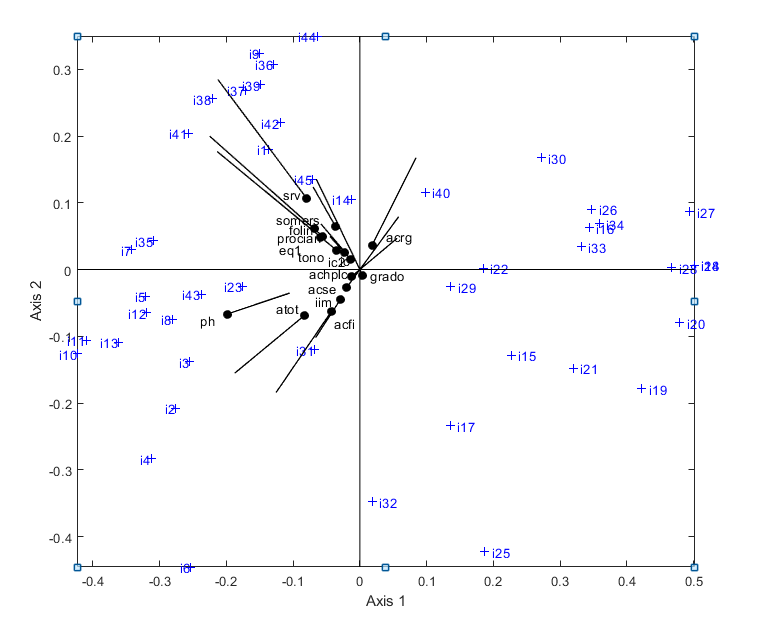
\includegraphics[width=0.75\linewidth]{LogBiplot} 

}

\caption{Biplot logístico}\label{fig:logbiplot}
\end{figure}

En el caso del biplot logístico mostrado en la figura 2, también se
puede deducir que la distribución de los individuos es diferente, pero
la contribución de las variables es diferente. Por ejemplo, el ph
contribuye a variables distintas. A pesar de ello, las direcciones de
los vectores de las variables como el somers, folin, y alrededor siguen
el mismo patrón.

\hypertarget{anuxe1lisis-canuxf3nico}{%
\subsection{Análisis Canónico}\label{anuxe1lisis-canuxf3nico}}

\begin{figure}

{\centering \includegraphics{biplot_files/figure-latex/disald-1} 

}

\caption{Función discriminante}\label{fig:disald}
\end{figure}

Mediante un análisis discriminante lineal, se obtiene la clasificación
de grupos tomando como referencia a cada una de las DDOO. La figura 3
muestra cómo el modelo logra clasificar correctamente a los dos grupos.

\begin{figure}
\centering
\includegraphics{biplot_files/figure-latex/canonico-1.pdf}
\caption{Biplot canónico discriminante}
\end{figure}

Prosiguiendo con el análisis MANOVA y su consecuencia proyección en el
biplot-total, la figura 4 muestra una clasificación similar a lo
detectado por el HJ-Biplot en el sentido en que los vinos Ribera del
Duero del 87 están claramente diferenciados del resto. Además de que los
vinos del Toro entre años tienen una variabilidad cercana, cuyo patrón
se puede rescatar de los otros dos métodos de biplot.

\hypertarget{discusiuxf3n}{%
\section{Discusión}\label{discusiuxf3n}}

Con los resultados de los análisis podemos deducir que aunque es posible
diferenciar las denominaciones de origen, los vinos Toro presentan
problemas de representación. En suma, cada método no es mejor que el
otro, sino herramientas útiles cuyo aprovechamiento depende del objetivo
de la investigación o respuesta que se quiera responder en cuanto al
documento. Queda en manifiesto que las técnicas biplot son una
representación gráfica poderosa que permite extraer información
relevante con precisión.

\hypertarget{referencias}{%
\section*{Referencias}\label{referencias}}
\addcontentsline{toc}{section}{Referencias}

\hypertarget{refs}{}
\leavevmode\hypertarget{ref-amaro2004}{}%
Amaro, Isidro Rafael, José Luis Vicente Vicente-Villardón, y Marı́a
Purificación Galindo-Villardón. 2004. «Manova Biplot para arreglos de
tratamientos con dos factores basado en modelos lineales generales
multivariantes». \emph{Interciencia} 29 (1): 26-32.

\leavevmode\hypertarget{ref-BERNABEU201377}{}%
Bernabéu, Rodolfo, Agustín Prieto, y Mónica Díaz. 2013. «Preference
patterns for wine consumption in Spain depending on the degree of
consumer ethnocentrism». \emph{Food Quality and Preference} 28 (1):
77-84.
\url{https://doi.org/https://doi.org/10.1016/j.foodqual.2012.08.003}.

\leavevmode\hypertarget{ref-callao1987}{}%
Callao, MP, J Guasch, MS Larrechi, y FX Rius. 1987. «Aroma components
and chemometric analysis to characterize catalan wine producing zones».
En \emph{Proceedings of II World Congress of Food Technology. E. Primo
and P. Fito (Eds.). Univ. Polit\textasciitilde{} cnica, Valencia,
Spain}.

\leavevmode\hypertarget{ref-ferranini2010}{}%
Ferrarini, R., C. Carbognin, E. M. Casarotti, E. Nicolis, A. Nencini, y
A. M. Meneghini. 2010. «The emotional response to wine consumption».
\emph{Food Quality and Preference} 21 (7): 720-25.
\url{https://doi.org/https://doi.org/10.1016/j.foodqual.2010.06.004}.

\leavevmode\hypertarget{ref-gabriel1971}{}%
Gabriel, Karl Ruben. 1971. «The biplot graphic display of matrices with
application to principal component analysis». \emph{Biometrika} 58 (3):
453-67.

\leavevmode\hypertarget{ref-greenacre1984}{}%
Greenacre, Michael J. 1984. «Theory and applications of correspondence
analysis».

\leavevmode\hypertarget{ref-mariani2012}{}%
Mariani, Angela, Eugenio Pomarici, y Vasco Boatto. 2012. «The
international wine trade: Recent trends and critical issues». \emph{Wine
Economics and Policy} 1 (1): 24-40.
\url{https://doi.org/https://doi.org/10.1016/j.wep.2012.10.001}.

\leavevmode\hypertarget{ref-mtimet2006}{}%
Mtimet, Nadhem, y Luis Miguel Albisu. 2006. «Spanish wine consumer
behavior: A choice experiment approach». \emph{Agribusiness} 22 (3):
343-62. \url{https://doi.org/10.1002/agr.20090}.

\leavevmode\hypertarget{ref-ogrinc_application_2003}{}%
Ogrinc, N., I. J. Košir, J. E. Spangenberg, y J. Kidrič. 2003. «The
application of NMR and MS methods for detection of adulteration of wine,
fruit juices, and olive oil. A review». \emph{Analytical and
Bioanalytical Chemistry} 376 (4): 424-30.
\url{https://doi.org/10.1007/s00216-003-1804-6}.

\leavevmode\hypertarget{ref-pyorala1990}{}%
Pyörälä, Eeva. 1990. «Trends in alcohol consumption in Spain, Portugal,
France and Italy from the 1950s until the 1980s». \emph{British Journal
of Addiction} 85 (4): 469-77.
\url{https://doi.org/10.1111/j.1360-0443.1990.tb01667.x}.

\leavevmode\hypertarget{ref-r2019}{}%
R Core Team. 2019. \emph{R: A Language and Environment for Statistical
Computing}. Vienna, Austria: R Foundation for Statistical Computing.
\url{https://www.R-project.org/}.

\leavevmode\hypertarget{ref-rivasgonzalo_etal_1993}{}%
Rivas-Gonzalo, Julián, V. Gutiérrez, A. Polanco, E. Hebrero, José Luis
Vicente-Villardón, Mª Purificación Galindo-Villardón, y C. Santos. 1993.
«Biplot Analysis Applied to Enological Parameters in the Geographical
Classification of Young Red Wines». \emph{American Journal of Enology
and Viticulture} 44 (enero): 302-8.

\leavevmode\hypertarget{ref-santa1986}{}%
Santa-Marı́a, G, JL Garrido, y C Diez. 1986. «The use of phenol compounds
as parameters for distinguished red and rose wines from pale wines in
multivariate analysis». \emph{Zeitschrift für Lebensmittel-Untersuchung
und Forschung} 182 (2): 112-14.

\leavevmode\hypertarget{ref-tapias1986}{}%
Tapias, RM, MS Larrechi, J Guasch, J Rubio, y FX Rius. 1986. «Enological
parameters and pattern recognition methods in the geographic
differentiation of Spanish red wines». \emph{American journal of enology
and viticulture} 37 (3): 195-201.

\leavevmode\hypertarget{ref-vasconcelos1989}{}%
Vasconcelos, Ana Maria P, y Higuinaldo J Chaves das Neves. 1989.
«Characterization of elementary wines of Vitis vinifera varieties by
pattern recognition of free amino acid profiles». \emph{Journal of
agricultural and food chemistry} 37 (4): 931-37.

\leavevmode\hypertarget{ref-vicente2014Multbiplot}{}%
Vicente-Villardón, J. L. 2014. «MULTBIPLOT: A package for Multivariate
Analysis using Biplots».
\url{http://biplot.usal.es/ClassicalBiplot/index.html}.

\leavevmode\hypertarget{ref-vicente2006}{}%
Vicente-Villardón, José L, M Purificación Galindo-Villardón, y Antonio
Blázquez-Zaballos. 2006. «Logistic biplots». \emph{Multiple
correspondence analysis and related methods. London: Chapman \& Hall},
503-21.

\leavevmode\hypertarget{ref-villardon1986}{}%
Villardón, Marı́a Purificación Galindo. 1986. «Una alternativa de
representacion simultanea: HJ-Biplot». \emph{Qüestiió: quaderns
d'estadı́stica i investigació operativa} 10 (1): 13-23.

\end{document}
